\section{原子性和持久性的实现}

数据库系统的恢复管理组件实现了对原子性和持久性的支持。

影子数据库方案——一种简单但效率低下的方案:一个名为db\_pointer的指针始终指向数据库的当前一致副本。

所有更新都在新创建的数据库副本上进行。原始副本——影子副本(影子拷贝)保持不变——由db\_pointer的指针始终指向数据库的当前一致副本。
\begin{itemize}
    \item 如果中止:只需删除新副本。
    \item 如果提交:1.将新副本内存中的所有页面写入磁盘(在Unix系统中,使用刷新命令)2.修改数据库指针,使其指向新副本——新副本成为当前副本,同时删除旧副本。
\end{itemize}

\begin{figure}[H]
    \centering
    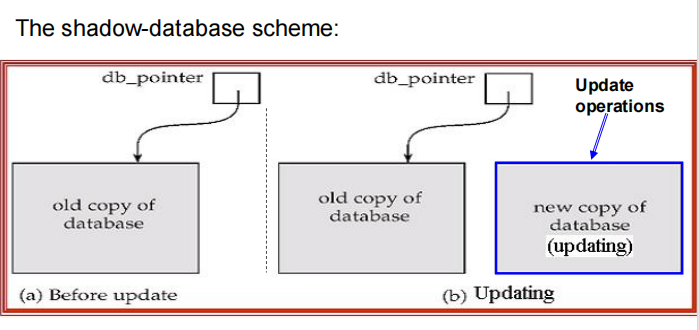
\includegraphics[width=0.8\linewidth]{image2.png}
    \caption{}
    \label{}
\end{figure}

\begin{figure}[H]
    \centering
    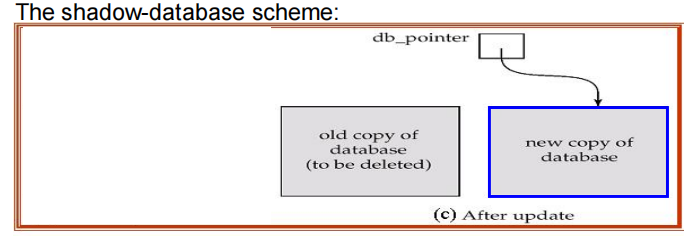
\includegraphics[width=0.8\linewidth]{image3.png}
    \caption{}
    \label{}
\end{figure}

要求:原子性地更新数据库指针(磁盘系统可保证这一点,将其存储在单个扇区中);无并发事务;假设磁盘不会发生故障。

这个想法对文本编辑器很有用。

但对于大型数据库而言效率极低;执行单个事务需要复值整个数据库。